\documentclass{standalone}

\usepackage{amsmath}
\usepackage{tikz}
\usetikzlibrary{calc, tikzmark, shapes, shapes.arrows, arrows, 3d, positioning}
\usepackage{bm}
\newcommand{\Omegahat}{\boldsymbol{\mathrm{\Omega}}}
\newcommand{\E}{\boldsymbol{\mathrm{E}}}
\newcommand{\ud}{\mathop{}\!\mathrm{d}} % upright derivative symbol
\renewcommand{\vec}[1]{\boldsymbol{#1}}

\begin{document}
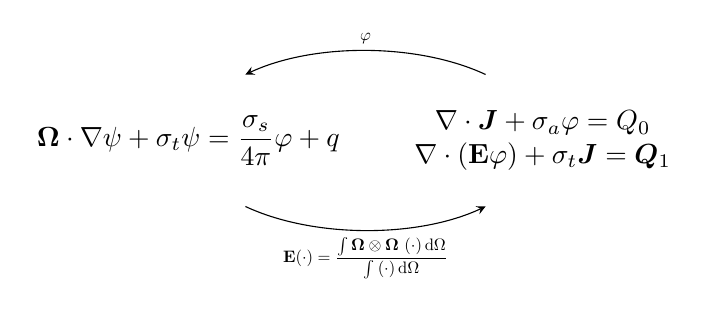
\begin{tikzpicture}
	\node (transport) at (0,0) {$\Omegahat\cdot\nabla\psi + \sigma_t \psi = \dfrac{\sigma_s}{4\pi}\varphi + q$}; 
	\node[align=center] (vef) at ([xshift=4.5cm]transport) {$\nabla\cdot\vec{J} + \sigma_a \varphi = Q_0$\\$\nabla\cdot\left(\E\varphi\right) + \sigma_t \vec{J} = \vec{Q}_1$}; 

	\draw[->, >=stealth, shorten <= 8mm, shorten >= 8mm] (transport |- {(0,-.5)}) to[bend right=25] node[midway, below=1mm, align=center, scale=.6] {$\E(\cdot) = \dfrac{\int \Omegahat\otimes\Omegahat\, \left(\cdot\right) \ud \Omega}{\int \left(\cdot\right)\ud \Omega}$} (vef |- {(0,-.5)});
	\draw[->, >=stealth, shorten <= 8mm, shorten >= 8mm] (vef |- {(0,.5)}) to[bend right=25] node[midway, above=1mm, align=center, scale=.6] {$\varphi$} (transport |- {(0,.5)});
\end{tikzpicture}
\end{document}